\section{Results}

\subsection{Brich3}
The output of the \texttt{kmeans.c} code is as follows.
\lstinputlisting[style=output]{output/brich.o}

Using this output following visualization is performed.
\begin{figure}[H]
    \centering
    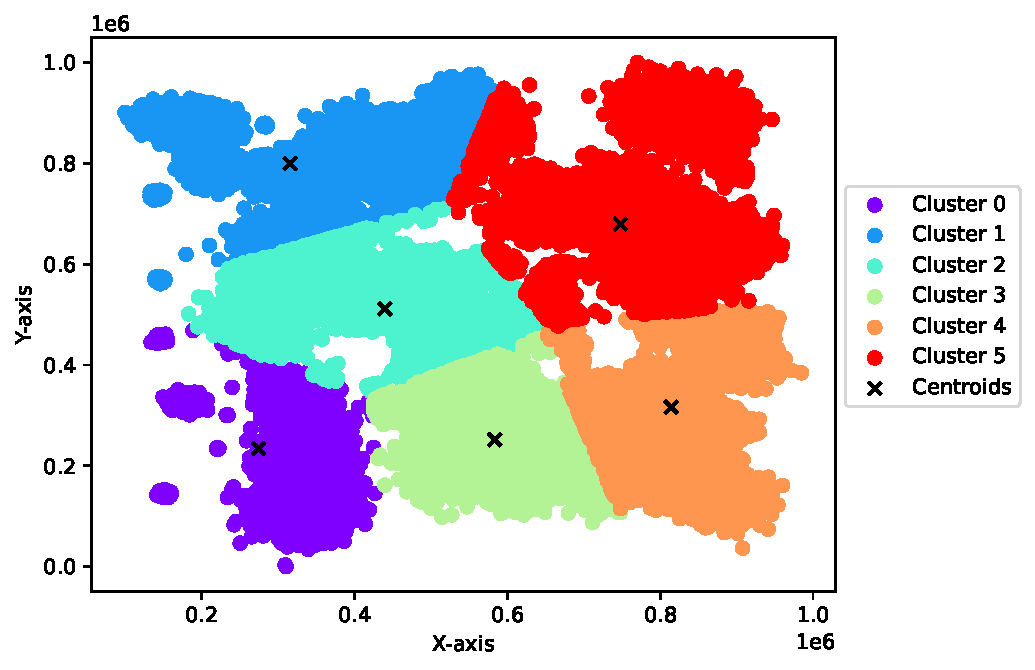
\includegraphics[width=.8\textwidth]{figures/brich.pdf}
    \caption{Brich3 N: 100000}
    \label{brich}
\end{figure}

\newpage
\subsection{Circle}
The output of the \texttt{kmeans.c} code is as follows.
\lstinputlisting[style=output]{output/circle.o}
Using this output following visualization is performed.

\begin{figure}[H]
    \centering
    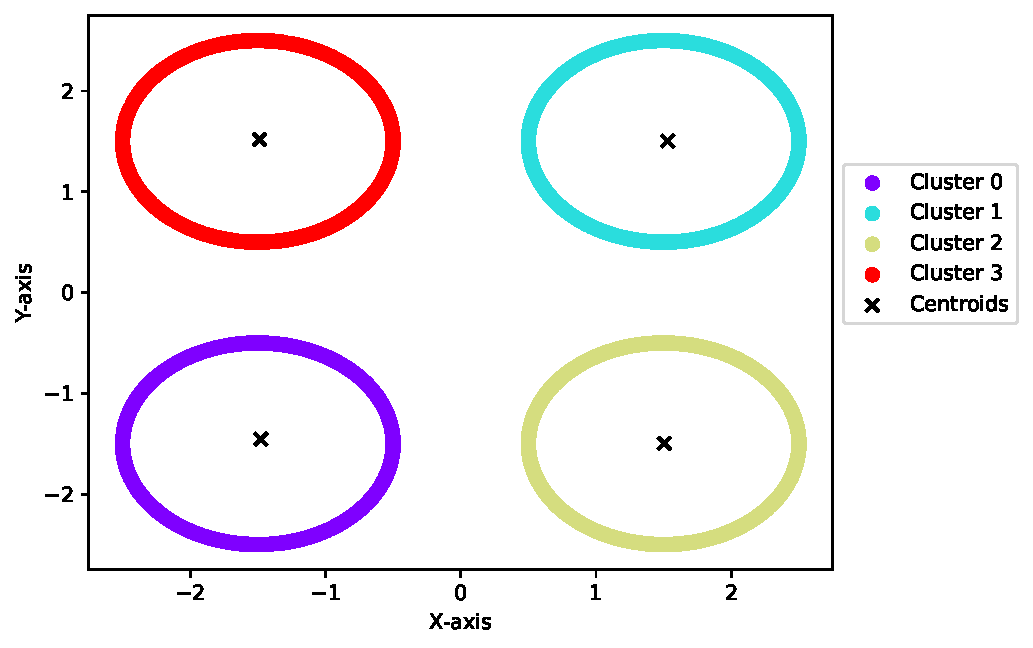
\includegraphics[width=.8\textwidth]{figures/circle.pdf}
    \caption{Circle N: 4000}
    \label{circle}
\end{figure}

\subsection{Hepta}
The output of the \texttt{kmeans.c} code is as follows.
\lstinputlisting[style=output]{output/hepta.o}

Using this output following visualization is performed.
\begin{figure}[H]
    \centering
    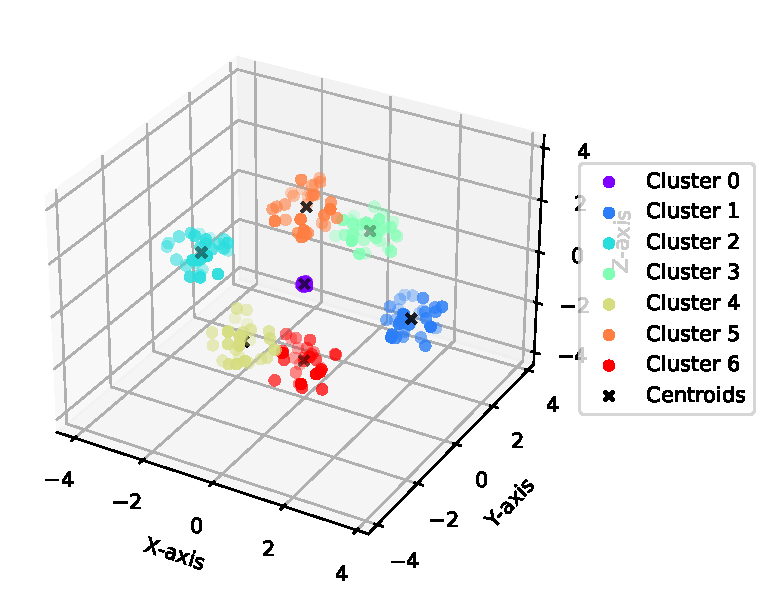
\includegraphics[width=.8\textwidth]{figures/hepta.pdf}
    \caption{Hepta N: 212}
    \label{hepta}
\end{figure}

\subsection{Isolation}
The output of the \texttt{kmeans.c} code is as follows.
\lstinputlisting[style=output]{output/isolation.o}

Using this output following visualization is performed.
\begin{figure}[H]
    \centering
    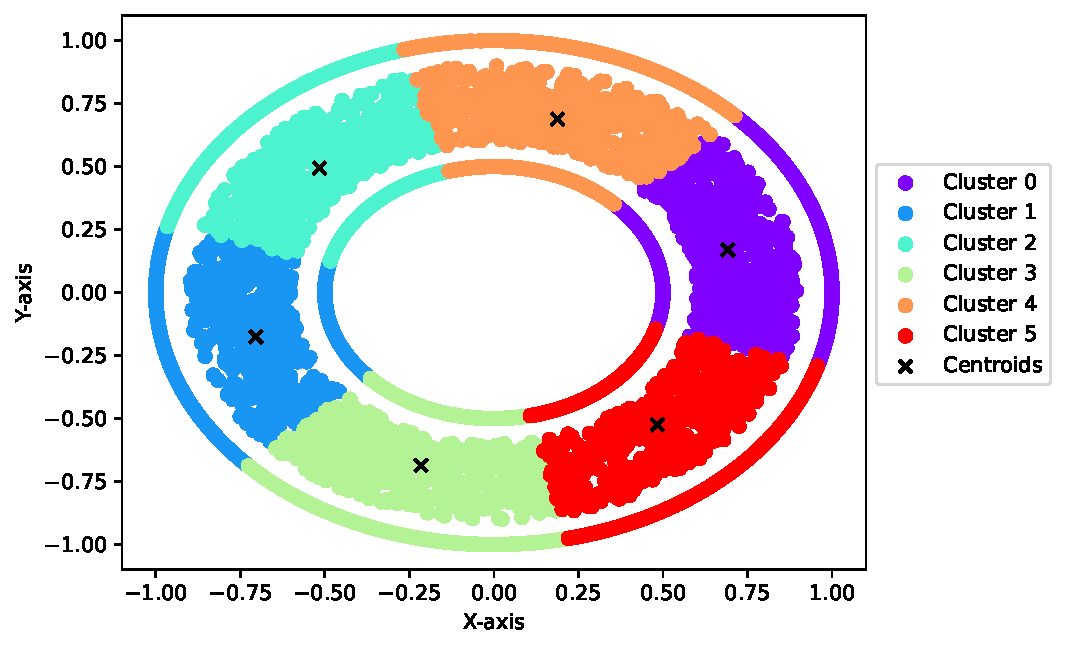
\includegraphics[width=.8\textwidth]{figures/isolation.pdf}
    \caption{Isolation N: 9000}
    \label{isolation}
\end{figure}

\subsection{Smile}
The output of the \texttt{kmeans.c} code is as follows.
\lstinputlisting[style=output]{output/smile.o}

Using this output following visualization is performed.
\begin{figure}[H]
    \centering
    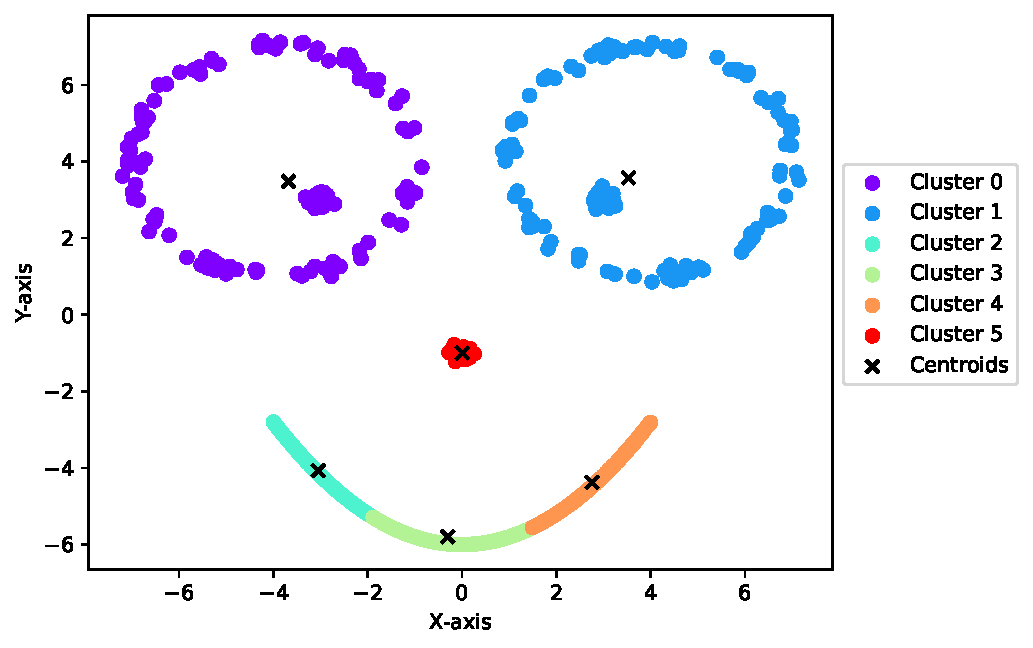
\includegraphics[width=.8\textwidth]{figures/smile.pdf}
    \caption{Smile N: 1000}
    \label{smile}
\end{figure}



